\chapter{The Optical Spring}
When detuned from resonance, the power circulating within a Fabry-Perot
cavity varies linearly with small deviations from that detuning. This
gives rise to a displacement-dependent force, which can be described
via a spring constant. This effect is called the \emph{optical spring}
\footnote{This is the longitudinal optical spring; an \emph{angular} optical spring
also arises, due to interactions between off-center radiation pressure and cavity geometry~\cite{Sidles2006Optical}.}.  Optical springs has been observed and studied in several experiments~\cite{Sheard2004Observation}.

For frequencies that are slow compared to the cavity pole, we can
calculate the behavior of the spring using a quasi-static approximation,
simply using the derivative of the power buildup versus cavity detuning.

The power circulating in a cavity is:
\begin{equation}
\frac{P_{+}}{P_{IN}}=\frac{g^{2}}{1+F\sin^{2}\phi}
\end{equation}
where $P_{IN}$ is the incident power, $P_{+}$ is the forward-circulating
power, $g^{2}=\left(t_{1}\right)^{2}/\left(1-r_{1}r_{2}\right)$ is
the power buildup on resonance, $F=4r_{1}r_{2}/\left(1-r_{1}r_{2}\right)^{2}$
is the coefficient of finesse%
\footnote{The finesse ($\mathcal{F}$) is related to the coefficient of finesse
($F$) via $\mathcal{F}\approx\frac{\pi}{2}\sqrt{F}$.%
}, and $\phi$ is the one-way phase detuning of the cavity, which is
related to cavity length $x$ as $\phi=(2\pi/\lambda)x$. 

For a given power circulating in the cavity, the radiation pressure
force due to the intra-cavity power on each of the mirrors is $f=2P/c$.
We can find the spring constant by taking the derivative:

\[
k\equiv-\frac{\partial f}{\partial x}=-\frac{\partial}{\partial x}\frac{2P}{c}=-\frac{2}{c}\frac{\partial\phi}{\partial x}\frac{\partial P}{\partial\phi}
\]
Working out the derivative, we find:

\begin{align}
\frac{\partial}{\partial\phi}P_{+} & =-2Fg^{2}\frac{\cos(\phi)\sin(\phi)}{\left(1+F\sin^{2}\phi\right)^{2}}P_{IN}\\
 & =-2Fg^{2}P_{IN}\phi+O\left(\phi^{3}\right)
\end{align}
Putting it all together, we get:
\begin{align}
k & =2Fg^{2}\left(\frac{2P_{IN}}{c}\right)\left(\frac{2\pi}{\lambda}\right)\frac{\cos(\phi)\sin(\phi)}{\left(1+F\sin^{2}\phi\right)^{2}}\label{eq:spring-constant}\\
 & \approx2Fg^{2}\left(\frac{2P_{IN}}{c}\right)\left(\frac{2\pi}{\lambda}\right)\frac{\phi}{\left(1+F\phi^{2}\right)^{2}}\label{eq:spring-constant-approx1}\\
 & \approx2Fg^{2}\left(\frac{2P_{IN}}{c}\right)\left(\frac{2\pi}{\lambda}\right)\phi+O\left(\phi^{3}\right)
\end{align}


where, of course, $\phi=(2\pi/\lambda)\delta x$, where $x$ is the
(one-way) detuning length. If a mirror is displaced by $(\delta x)$,
the spring constant is:
\[
k\approx\frac{64\mathcal{F}^{2}g^{2}P_{IN}}{c\lambda^{2}}\left(\delta x\right)
\]
Putting in some numbers for the Enhanced LIGO arms:
\begin{align*}
\mathcal{F} & =220\\
g^{2} & =137\\
P_{IN} & =400\mathrm{\ Watts}\\
\lambda & =1064\mathrm{\ nm}\\
\delta x & =5\mathrm{\ pm}\\
\hline k & \approx2500\mathrm{\ N/m}
\end{align*}
For comparison, the mechanical restoring force has a spring constant
of approximately
\[
k_{m}=m\omega^{2}\approx\left(10.5\text{ kg}\right)\left(2\pi\cdot0.7\text{5 Hz}\right)^{2}\approx230\text{ \ensuremath{\frac{\text{N}}{\text{m}}}}
\]


It can also be handy to put Eq. \ref{eq:spring-constant-approx1}
into terms of the unitless detuning parameter $\delta_{\gamma}=\sqrt{F}\phi$,
where $\delta_{\gamma}\equiv\frac{\delta}{\gamma}$, where $\delta$
is the cavity detuning (in radians/sec), and $\gamma$ is the line-width
(cavity pole) in the same units. If we further assume that the cavity
is strongly-overcoupled, we can use the relations $g^{2}=\sqrt{F}=\frac{2}{\pi}\mathcal{F}=4/T_{1}$.
With these substitutions (and $\lambda=2\pi c/w_{0}$), we recover
expression (3.14) given in Thomas Corbitt's thesis \cite{Corbitt2008Quantum}:
\begin{equation}
K_{0}\approx\frac{64P_{IN}w_{0}}{T^{2}c^{2}}\frac{\delta_{\gamma}}{\left(1+\delta_{\gamma}^{2}\right)^{2}}
\end{equation}


\section*{Coupled oscillators}

Consider a system of two masses, connected to each other via a spring
with spring constant $k_{1}$ and each connected to the wall via a
spring of spring constant $k_{0}$. (Later, $k_{0}$ will represent
the pendula by which the optics are suspended, and $k_{1}$ will represent
the optical spring.)

\begin{center}
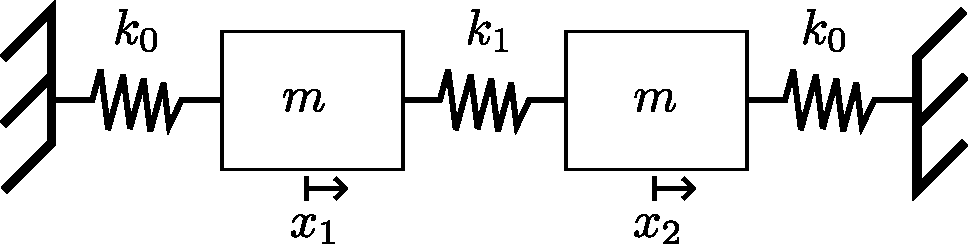
\includegraphics[width=0.4\paperwidth]{figures/coupled-oscillators-diagram}
\par\end{center}

By inspection, the equations of motion are:
\begin{eqnarray}
m\ddot{x}_{1} & = & -k_{0}x_{1}+k_{1}(x_{2}-x_{1})\\
m\ddot{x}_{2} & = & -k_{0}x_{2}-k_{1}(x_{2}-x_{1})
\end{eqnarray}
which may be written in matrix form as
\begin{equation}
\mathbf{\ddot{x}}=\frac{1}{m}\left[\begin{array}{cc}
-(k_{0}+k_{1}) & k_{1}\\
k_{1} & -(k_{0}+k_{1})
\end{array}\right]\mathbf{x}
\end{equation}
Because of the form of the matrix%
\footnote{The matrix $\left[\begin{array}{cc}
a & b\\
b & a
\end{array}\right]$ has eigenvectors $\left(\begin{array}{c}
1\\
1
\end{array}\right)$ and $\left(\begin{array}{c}
1\\
-1
\end{array}\right)$ with eigenvalues $(a+b)$ and $(a-b)$.%
}, we can immediately see that it has eigenvectors corresponding to
common and differential motion, with eigenvalues $\left\{ -k_{0},-(k_{0}+2k_{1})\right\} $. 

Applying this diagonalization, we find:
\[
\mathbf{\ddot{x'}}=\frac{1}{m}\left[\begin{array}{cc}
-k_{0} & 0\\
0 & -(k_{0}+2k_{1})
\end{array}\right]\mathbf{x'}\text{ where }\mathbf{x'}=\left[\begin{array}{cc}
1 & 1\\
1 & -1
\end{array}\right]\mathbf{x}
\]
The presence of the coupling $k_{1}$ only affects the differential
mode.


%% \subsection{Damped oscillators}

%% Now consider a mass connected to the wall via a spring with spring
%% constant $k$ and a velocity damper with damping constant $\gamma$:

%% \begin{center}
%% 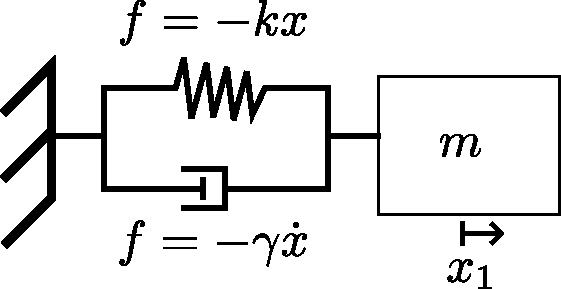
\includegraphics[width=0.25\paperwidth]{figures/damped-oscillator-diagram}
%% \par\end{center}

%% The equation of motion of the mass is:
%% \begin{equation}
%% m\ddot{x}=-kx-\gamma\dot{x}+f_{external}
%% \end{equation}
%% with Laplace transform
%% \begin{equation}
%% ms^{2}X=-kX-\gamma sX+F_{external}
%% \end{equation}
%% giving rise to a transfer function of

%% \begin{eqnarray*}
%% \frac{X}{F} & = & \frac{1}{ms^{2}+\gamma s+k}\\
%%  & = & \left(\frac{1}{m}\right)\frac{1}{\left(s-s_{+}\right)\left(s-s_{-}\right)}\text{ with }s_{\pm}=-\frac{1}{2}\frac{\gamma}{m}\pm\frac{1}{2}\sqrt{\left(\frac{\gamma}{m}\right)^{2}-4\frac{k}{m}}
%% \end{eqnarray*}


%% \subsection{Optical damping}

%% Suppose the cavity mirrors are traveling away from each other with
%% a velocity $v$. Then the phase of the reflected beam is changing
%% at a rate $\left(2\pi/\lambda\right)2v$. We can interpret this as
%% the light being Doppler shifted by $\Delta\omega=\left(2\pi/\lambda\right)2v$.
%% This optical frequency shift will cause the cavity to be closer or
%% further to resonance as compared to a cavity with stationary mirrors.

%% From this we can calculate the optical damping coefficient $\gamma$:

%% \[
%% \gamma\equiv-\frac{\partial f}{\partial v}=-\frac{\partial}{\partial v}\frac{2P}{c}=-\frac{2}{c}\frac{\partial\phi}{\partial v}\frac{\partial P}{\partial\phi}
%% \]
%% where $\frac{\partial\phi}{\partial v}=\frac{\partial\phi}{\partial\omega}\frac{\partial\omega}{\partial v}=\left(1/fsr\right)\left(4\pi/\lambda\right)$
%% so
%% \[
%% \gamma=\frac{2}{c}\frac{1}{fsr}\frac{4\pi}{\lambda}2Fg^{2}\frac{\cos(\phi)\sin(\phi)}{\left(1+F\sin^{2}\phi\right)^{2}}P_{IN}
%% \]

\begin{figure}
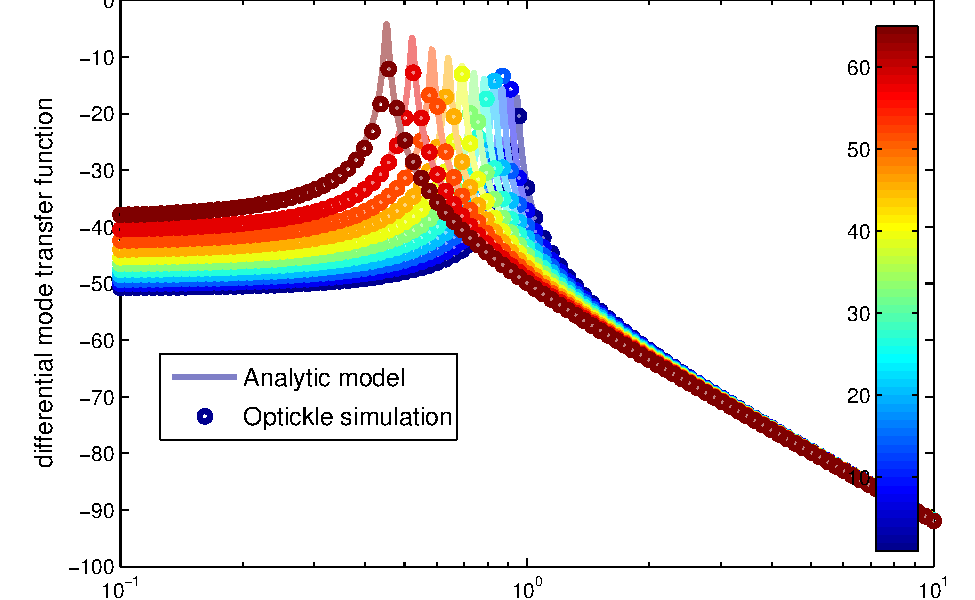
\includegraphics[width=\columnwidth]{figures/model-comparison}
\caption[Optical spring transfer function (numerical and analytic)]{\label{fig:model-comparison}The optical spring effect:  As a cavity is detuned from resonance, the resonance of the differential mode deceases.  This figure compares the resultsof a numerical  (Optickle) model with analytic results. The units of the
  y-axis are $20\log_{10}$(displacement/force); the x-axis is Hz;
  color indicates cavity detuning in picometers.}
\end{figure}
